\begin{figure}[ht]
  \centering
  \subfigure[]{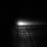
\includegraphics[width=4cm,keepaspectratio]{interference/figures/move/321-1.jpg}}
  \subfigure[]{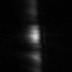
\includegraphics[width=4cm,keepaspectratio]{interference/figures/move/321-2.jpg}}
  \subfigure[]{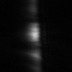
\includegraphics[width=4cm,keepaspectratio]{interference/figures/move/321-3.jpg}}\\
  \subfigure[]{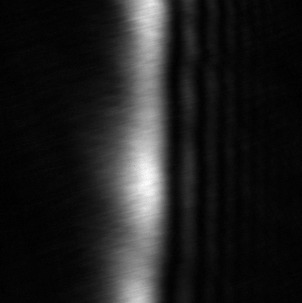
\includegraphics[width=4cm,keepaspectratio]{interference/figures/move/321-7.jpg}}
  \subfigure[]{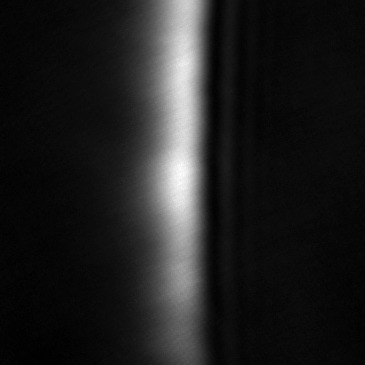
\includegraphics[width=4cm,keepaspectratio]{interference/figures/move/321-8.jpg}}
  \subfigure[]{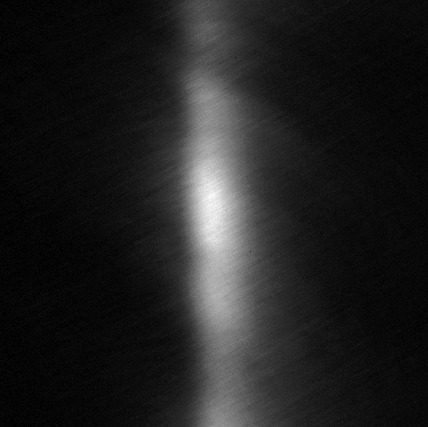
\includegraphics[width=4cm,keepaspectratio]{interference/figures/move/321-9.jpg}}\\
  \caption{Images of the optical field for the section of the conically
    scattered light as the focal plane of $f_4$ is moved from (a), best focus,
    to (f), the far field.  All images have been normalized relative to
    themselves.}\label{fig:321up}
\end{figure}
